\chapter{Automatización de la gestión de aparcamientos para PMR}
Como se ha visto anteriormente, ya se ha analizado el proyecto desde un punto de vista legislativo. En este capítulo se va a definir qué funcionalidades, requisitos y restricciones tiene que tener un sistema ideal que dé solución a los problemas expuestos en las plazas de aparcamiento para PMR.
\\\\
Al describir las funcionalidades, requisitos y restricciones del sistema se quiere conseguir hacer un análisis más detallado de lo que sería realmente el sistema. Esto, que realmente son especificaciones que cualquier persona podría entregar a un ingeniero, es el primer paso para la elaboración de cualquier sistema informático.
\\\\
Para poder definir las funcionalidades del sistema, es necesario definir primero los usuarios del mismo, debido a que son éstos los que interactúan con el sistema. En primera instancia, hay dos tipos de usuarios: los usuarios finales que hacen uso de las plazas de aparcamiento y los administradores del sistema que se encargan de su configuración. 
\\\\
Ya se ha comentado anteriormente que el usuario final de este sistema podrá ver el estado de las plazas en tiempo real y navegar a la plaza disponible más cercana a una dirección. Pero, para ello, es necesario que se coloquen plazas en la vía pública, que se controlen y que se den de alta a estos usuarios finales. Dichas acciones de gestión interna del sistema las hacen organismos independientes.
\\\\
La colocación de las plazas en la vía pública de un municipio o ciudad es competencia del consistorio de la misma. Por otro lado, el control viene dado por la autoridad del municipio (e.g. policía local). Así mismo, continuando con los organismos que tienen que ver con las plazas para PMR, los organismos que expiden la acreditación de aparcamiento al usuario son las comunidades autónomas. Esta información proviene del marco legal visto anteriormente y hace que, dependiendo del organismo, se tenga que concebir o restringir el uso de funcionalidades del sistema a los administradores de los distintos organismos.
\\\\
Por supuesto, alguna de la información almacenada y tratada por el sistema va a ser información confidencial y de carácter personal por lo que el acceso de cada persona que haga uso del sistema deberá quedar registrado. Esto hace que el sistema se pueda auditar correctamente si se necesita.
\\\\
Además de las personas que van a interactuar con el sistema, algunos de sus componentes interactúan automáticamente entre ellos. Dichos componentes se definen como agentes y, al igual que los usuarios, consultan, modifican, añaden o eliminan información del sistema. Un ejemplo más palpable de estos agentes son los encargados de captar datos en las distintas plazas de aparcamiento e informar al sistema sobre el estado de las mismas.
\\\\
Resumiendo, hay distintos tipos de usuarios: \textit{usuarios finales} que hacen uso de las plazas, \textit{administradores} (consistorio, autoridad de control y CCAA) que gestionan todo lo que tiene que ver con las plazas y \textit{agentes} que son componentes del sistema. Una vez que se conocen los diferentes usuarios que van a interactuar con el sistema, se puede empezar a citar algunas de las funcionalidades de los mismos. 
\section{Funcionalidad general deseable}
Ahora, al saber los usuarios que interactuarán con el sistema, es el momento de pensar y citar qué funcionalidades son las deseadas para cada uno de estos tipos de usuarios. Las funcionalidades no son más que una serie de características del sistema que resuelven, de forma útil, un objetivo del usuario. Para citarlas, es mejor agruparlas dependiendo del usuario del sistema.
\subsection{Usuarios finales}
Los usuarios finales interactuarán con el sistema, principalmente, a través de una aplicación móvil mientras que están conduciendo un vehículo. Adicionalmente, podrán interactuar con el sistema a través de una plataforma web desde cualquier dispositivo que disponga de un navegador.
\\\\
A su vez, estos usuarios podrán o no estar registrados en el sistema. Si no se encuentran registrados, las funcionalidades asociadas se verán restringidas por motivos de seguridad y de modelo de negocio. Por lo que para que un usuario disponga de todas las funcionalidades posibles, deberá registrarse.
\\\\
La funcionalidad principal que debiera tener el usuario, que hace uso de los aparcamientos tratados, es poder visualizar en el mapa de un municipio la localización de las distintas plazas de aparcamiento y navegar hacia una de ellas. Esta información es pública por lo que cualquier usuario de este sistema tendría que tener acceso desde cualquier dispositivo.
\\\\
Este sistema no se basa en sólo saber dónde se encuentran las distintas plazas de aparcamiento, sino también saber su estado de ocupación. El usuario final, si se encuentra registrado en el sistema, debería poder consultar dicho estado para poderse hacer una idea de en qué plaza aparcará. Este estado lo vería como “disponible” si la plaza está libre, “ocupada” si la plaza se encuentra ocupada por un vehículo con autorización, “mal ocupada” si la plaza se encuentra ocupada por un vehículo sin autorización y “aviso a grúa” si el vehículo mal aparcado está esperando para ser retirado, por lo que tendrá una mejor idea al buscar aparcamiento.
\\\\
No obstante, si se encuentra conduciendo, el proceso de ver un mapa en el móvil y buscar una plaza de aparcamiento es peligroso, a la vez que ilegal (artículo 13 del Real Decreto Legislativo 6/2015, de 30 de octubre, por el que se aprueba el texto refundido de la Ley sobre Tráfico, Circulación de Vehículos a Motor y Seguridad Vial \cite{rdl6-2015}). Por ello, la aplicación móvil debería ser capaz de buscar una plaza de aparcamiento de igual forma que el usuario lo haría. Para que el sistema sea capaz de encontrar la plaza más idónea, es necesario que el usuario le informe de un destino y una serie de preferencias. A través de dicho destino, el sistema, contando con la ocupación de las plazas y si el usuario se encuentra registrado, mostrará un listado de las mejores plazas donde aparcar su vehículo.
\\\\
Aquí también se tendrán en cuenta necesidades especiales del usuario en el momento de buscar aparcamiento de igual manera que el usuario haría. Dichas necesidades pueden ser tener en cuenta la diferencia de altitud entre la plaza y el destino, si el usuario se desplaza en silla de ruedas manual, o el tamaño y tipo de aparcamiento, si el usuario necesita salir del vehículo por la parte posterior en una silla de ruedas motorizada.
\\\\
Si el usuario, sea de forma manual o automática, busca una plaza y la selecciona, la aplicación tendría que poder guiar al usuario a dicha plaza. La forma de guiarle sería con señales acústicas y visuales durante el recorrido hasta llegar a la plaza indicada. Para ello, la aplicación móvil hará uso del GPS del dispositivo, así como avisará al usuario si, durante el trayecto, la plaza deseada se ha ocupado.
\\\\
Una vez el usuario se encuentra en una plaza y vea algún tipo de incidencia en la misma (vehículo mal aparcado, daños en las señalizaciones, daños en las vías de acceso a las plazas, imposibilidad de aparcar…) podrá avisar a la autoridad de control desde la propia aplicación quedando dicha incidencia doblemente registrada, en este sistema y en el sistema externo de la autoridad. También, si lo desea y está dado de alta en el sistema, podrá valorar el estado de las plazas donde aparque. 
\\\\
Dichas valoraciones servirán para mejorar el estado de las plazas teniendo en cuenta su accesibilidad, ubicación, tamaño, señalización…, así como comentarios sobre ella. Además, pueden servir a otros usuarios para filtrar, a través de estas valoraciones, plazas o zonas de aparcamiento al buscar uno.
\subsection{Administradores}
Cada organismo necesita administrar una parte del sistema, según la normativa vigente vista en el marco legal de estas plazas. Cada uno de estos tendrán un conjunto de funcionalidades distintas pero no disjuntas, debido que a hay funcionalidades compartidas entre organismos distintos como se verá en detalle.
\subsubsection{Consistorio o ayuntamiento}
Es el organismo que tiene potestad para poner o quitar plazas de su municipio. Debido a dicha potestad tendría que dar de alta o baja plazas de aparcamiento en tu término municipal. Se sabe que en algunos casos se sitúa más de una plaza en la misma ubicación y en otros hay plazas sueltas, con alguna restricción horaria. También se puede dar la posibilidad de que la plaza la pueda compartir una PMR con otros vehículos autorizados como pueden ser sanitarios o de autoridad.
\\\\
Por otra parte, una vez colocadas las plazas, desde el ayuntamiento se deberían consultar estadísticas de ocupación de las plazas de aparcamiento para así mejorar el número de plazas o la ubicación de las mismas. A su vez, se debería poder consultar estadísticas de las valoraciones que los usuarios hacen de las plazas de aparcamiento que utilizan, así como de sus comentarios y las incidencias que ocurren en ellas. Estas estadísticas tendrían que verse anonimizadas, es decir, no se debería saber la valoración de un usuario en concreto.
\\\\
También, como el sistema debiera registrar los destinos de los usuarios que utilizan el sistema, se debería poder consultar cuáles son los destinos más usuales para una mejor ubicación de las plazas. Dichos destinos, de igual forma que los datos anteriores, estarían anonimizados. De esta manera se preserva la identidad de los usuarios del sistema haciendo que sea más seguro.
\subsubsection{Autoridad de control}
La autoridad solo necesita disponer de la información relativa a la ocupación de las plazas proveniente de los agentes de captación de datos del sistema y a las incidencias provenientes de los usuarios. Con esta información podrían recibir notificaciones en tiempo real de las plazas donde se está cometiendo algún tipo de infracción. 
\\\\
Una vez recibidas notificaciones del sistema en la unidad central de la autoridad competente (Policía Local), se tratarían estas notificaciones creadas de forma automática por el sistema o manual por los usuarios del mismo como si fuese una llamada, quedando registrada en el sistema de gestión automática de estas plazas como en el sistema de la autoridad.
\\\\
Al tener una notificación de una incidencia en una plaza para PMR, se debería hacer una supervisión humana de la incidencia. Al hacerla puede resultar que la autoridad de control tenga que proceder a la retirada del vehículo de la plaza de aparcamiento. Si esto sucede, tendría que modificar el estado de la plaza de ``mal ocupada'' a ``aviso a grúa'' para que el sistema y los usuarios tengan una mayor información sobre cuándo se puede quedar disponible la plaza.
\\\\
Del mismo modo que el ayuntamiento, la autoridad de control debería poder tener acceso a estadísticas de ocupación donde poder ver qué plazas o zonas del municipio tienen un mayor grado de incidencias para aumentar el control en dichas zonas.
\subsubsection{Comunidades autónomas}
Las CCAA son las encargadas, en España, de expedir las tarjetas que autorizan el estacionamiento en las plazas para PMR. Es por este motivo que su funcionalidad principal sería dar de alta o baja a usuarios para que estos puedan hacer uso de las plazas debido a que necesitan estar registrados en el sistema.
\\\\
A su vez, las CCAA deberían dar de alta a los municipios que deseen utilizar este sistema creando los dos perfiles necesarios para ello: ayuntamiento y autoridad de control.
\subsection{Agentes software}
Los agentes son componentes del sistema que tienen la capacidad de interactuar con el mismo y entre ellos. Como se ha dicho, un ejemplo de estos son los encargados de captar datos para que el sistema sepa, sin intervención humana, el estado de ocupación de una plaza.
\\\\
Para ello, los agentes de captación de datos tienen que ser capaces de distinguir cuándo una plaza de aparcamiento se encuentra libre u ocupada. También si se encuentra ocupada, saber si el vehículo estacionado presenta acreditación o no. Esto hace que estos agentes sean pieza fundamental en este sistema, debido a que son los encargados de hacer que los datos, con los que el sistema trabaja, sean veraces y en tiempo real.
\\\\
Otro tipo de agentes que podría tener el sistema serían los encargados de buscar una plaza de aparcamiento de forma similar a la que el usuario lo haría.  Estos agentes tendrían una componente de inteligencia artificial (IA) mayor. Éstos tendrían que usar datos de configuración introducidos por el usuario como puede ser el destino donde quiera ir, preferencias para una plaza marcadas por sus necesidades, así como los datos de ocupación de las plazas. Con esto, el agente inteligente podría recomendar la mejor plaza al usuario de una forma más rápida y concisa del que este lo haría.
\section{Restricciones}
Lo que se ha visto anteriormente serían algunas de las funcionalidades deseadas que el sistema debiera tener. No obstante, si se quiere llevar a cabo este sistema ideal en un ambiente real (por ejemplo, el marco de este TFG), se tiene que hacer frente a una serie de restricciones técnicas y no técnicas que van a dificultar la labor de encontrar una solución tangible.
\\\\
En primer lugar, antes de desarrollar el proyecto, hay que marcar un presupuesto máximo razonable ya que, de otra manera, no sería posible su implantación. Aquí, además de contar con un presupuesto para el desarrollo software y el desarrollo del sistema, el presupuesto del agente de captación de datos es muy importante debido a que es el ayuntamiento quien tiene que costear la colocación de estos agentes y el hardware que los sustenta en la vía pública. Además, con respecto al marco legal, los agentes de captación de datos, al estar en la vía pública, tienen que cumplir las normativas establecidas para poder ser colocados.
\\\\
Siguiendo con el marco legal, el sistema almacenará y tratará con datos de carácter personal. Aquí la normativa vigente es muy estricta. Esto repercute en el desarrollo del software debido a que tiene que ser un desarrollo muy seguro. Todos los accesos al sistema deberán ser registrados a la vez que, si es necesario, se pueda auditar el sistema de una forma correcta.
\\\\
También, las comunicaciones deberán estar cifradas y autenticadas para impedir el robo de información a través de estos canales. Por otro lado, el sistema deberá disponer de un subsistema de información redundante para evitar la pérdida de información por algún tipo de fallo ya sea software o hardware. Así, además de evitar un problema de seguridad o legalidad (datos de carácter personal), se evita a su vez un problema de fiabilidad debido a que, si hay algún fallo, el sistema seguiría trabajando de forma normal.
\\\\
Además de usar sistemas de información redundantes, la captación de esta información por parte de los agentes debiera ser también redundante para evitar fallos de información en el sistema, es decir, si no se capta un vehículo, la disponibilidad de la plaza sería errónea con lo que el sistema no funcionaría correctamente.
\newpage
\section{Estudio preliminar}
Al conocer ya algunas de las funcionalidades y de las restricciones del sistema, se va realizar a un estudio del sistema para poner todo en conjunto. Esto hace que se tenga una visión más clara del sistema a la vez que se le da forma general al mismo. 
\\\\
Por lo que se ha hablado hasta ahora, el sistema se puede dividir en tres \textit{capas}:
\begin{itemize}
	\item en la primera se encuentran los agentes encargados de la captación de datos que hacen que la información con la que trabaja el sistema sea veraz.
	\item la segunda se compone del almacenamiento y el tratamiento de la información. Aquí será el lugar para ubicar los agentes inteligentes, así como todo el procesamiento de datos para que los usuarios puedan, por ejemplo, acceder a estadísticas.
	\item la tercera son las distintas aplicaciones para que los usuarios interactúen con el sistema. Como ya se ha mencionado, habrá una aplicación móvil y plataforma web para el usuario final, otra aplicación móvil para la autoridad de control y una aplicación de escritorio, que dependiendo del usuario que acceda en ella, mostrará funcionalidades de gestión para los distintos tipos de administradores.
\end{itemize}
Con respecto a la tercera capa, la creación de las distintas aplicaciones va a depender exclusivamente de un aspecto técnico al escoger, de las distintas tecnologías posibles, una que por robustez u otros aspectos se considere la mejor para ello. Esta elección se detallará más adelante en el análisis software de la solución.
\\\\
La segunda capa se tiene que definir una vez analizada la anterior ya que, en este punto, el almacenamiento y el tratamiento de la información se podría hacer de forma distribuida.
\\\\
Por tanto, adquiere especial relevancia la resolución del problema de captación de datos, la primera capa de las tres mencionadas. Este hecho repercutirá en todo el sistema ya que es una parte fundamental y es el vínculo de conexión entre la lógica del sistema y la realidad que se quiere solventar.
\newpage
\subsection{Captación de datos} \label{captacion}
Como se ha comentado anteriormente, los agentes encargados de la captación de datos de las plazas de aparcamiento son un pilar fundamental en este sistema. Debido a ello, esta capa es la que más restricciones tiene. Por un lado, los agentes tienen que tener un presupuesto ajustado en lo posible para permitir la implantación del sistema en cualquier municipio. Esto también afecta al mantenimiento de los mismos, debido a que un mayor mantenimiento eleva el presupuesto del sistema.
\\\\
Por otro lado, se encuentran las restricciones legales al estar situados en la vía pública, debido a que tienen que garantizar que las ordenanzas se cumplan, así como ser un objeto pasivo que no pueda causar daños a viandantes ni a los propios vehículos. También, las comunicaciones entre los distintos dispositivos deberán ser seguras, al igual que el propio agente, para impedir el robo de información o una supuesta filtración en el sistema.
\\\\
Por último, estos agentes presentan restricciones técnicas al deber captar la ocupación de una plaza a la vez que, si la plaza se encuentra ocupada, controlar si el vehículo presenta autorización o no. Esta captación debe ser pasiva, redundante y segura para que sea lo más fiable posible y cumpla con las restricciones legales. Además, al estar situados a la intemperie, los agentes deberían ser lo más robustos posibles ya que estarán expuestos a inclemencias meteorológicas, basura o vandalismo.
\\\\
Es por ello que el primer agente de captación de datos en el que se pensó fueron las cámaras de tráfico y/o de seguridad implantadas en los municipios o ciudades. Con ello, se reduce a nulo la partida presupuestaria para implantar el sistema, siendo las cámaras capaces de distinguir una acreditación de aparcamiento en la luna delantera del vehículo. También, las restricciones se reducirían al no tener que implantar nada nuevo.
\\\\
Aunque no habría restricciones legales de implantación, el hecho de acceder a todas las cámaras de una ciudad para comprobar la ocupación de aparcamientos es inviable por razones de seguridad o confidencialidad. Además, habría que filtrar qué cámaras visualizan los aparcamientos que en este proyecto se tratan, hecho que se debería automatizar aumentando la complejidad de la parte técnica y su presupuesto asociado.
\\\\
También, de hacerlo así, habría plazas de aparcamiento que no podrían ser visualizadas por lo que la información del sistemas sería parcial y poco fiable. Tampoco se podría visualizar correctamente la tarjeta acreditativa de aparcamiento porque dependerá de cómo se aparque el vehículo. Todos estos aspectos hacen que se rechace el uso de las cámaras de tráfico o de seguridad como agentes de captación de datos.
\\\\
Siguiendo con la filosofía de usar cámaras como agentes de captación de datos con la idea de poder visualizar la tarjeta de acreditación de aparcamiento, se pensó en desplegar cámaras en las plazas de aparcamiento que se quieren controlar. Este cambio hace que se tenga acceso a los datos y se sepa que todos ellos visualizan plazas a controlar por lo que bajaría la complejidad técnica y el sistema dispondría de una información correcta y completa de la realidad.
\\\\
Por otro lado, el presupuesto de este sistema sería desorbitado debido a que las cámaras deberían tener visión nocturna para que el sistema siga funcionando con poca luz. A esto se le suma que el sistema de captación no serviría si el vehículo estaciona de forma diferente en la plaza debido a que, la cámara no visualizaría la tarjeta de aparcamiento por lo que se producirían errores de fiabilidad en los datos del sistema. De igual modo, si el vehículo aparca muy cerca de la cámara, esta se taparía y no podría realizar su función. Algo similar ocurriría si se tapa la cámara de manera intencionada, con lo que debería tenerse en cuenta el presupuesto de mantenimiento.
\\\\
Hasta ahora se ha pensado en cámaras para poder captar la tarjeta de acreditación para el uso de los aparcamientos para PMR. Esto ha incrementado de manera notoria el presupuesto del sistema no teniendo, algunas veces, información fiable de la realidad, por lo que el sistema no serviría.
\\\\
Debido a ello, se tiene que dar un cambio de paradigma o perspectiva para solucionar este problema y minimizar el presupuesto de implantación del sistema. Este cambio pasa por que la tarjeta acreditativa de aparcamiento se pueda percibir por algún otro medio que no sea visual. Con esto se cambia de un tipo de sensor en concreto, cámaras, a cualquier tipo de sensor.
\\\\
Antes de detenerse en el proceso de detección del vehículo se deberá adoptar una solución para la tarjeta de aparcamiento. La solución tiene que ser lo más económica posible y el usuario de estos aparcamientos debería seguir sus costumbres habituales.
\\\\
Por eso, cualquier aparato nuevo que acompañe a la tarjeta acreditativa y necesite de batería queda automáticamente descartado. Estos dispositivos pueden ser de tipo Bluetooth (BLE) donde haya un emisor en el vehículo y un receptor en las distintas plazas de aparcamiento. Aunque estos dispositivos tienen un coste despreciable, el hecho de que necesiten una fuente de energía hace que el usuario se tenga que preocupar por el dispositivo ya que también, debería ser portable como la tarjeta de aparcamiento.
\\\\
La solución sería incluir en la propia tarjeta el dispositivo. Éste no debería tener fuente de alimentación propia por lo que suponen muchas restricciones para elegir el dispositivo. El único viable que cumple todas estas restricciones es la tecnología RFID. 
\\\\
Esta tecnología, actualmente, se encuentra en multitud de productos que la sociedad maneja diariamente como billetes de metro o autobús, tarjetas de organismos o bancos e incluso, son las alarmas de muchos productos de tiendas. Lo más caro de esta tecnología es el receptor de información que es una bobina que crea un campo electromagnético. No obstante tendría un presupuesto muy aceptable para su implantación.
\\\\
Ahora que se ha resuelto el problema de la detección de la tarjeta de aparcamiento a través de sensores, es hora de detectar un vehículo a través de sensores de igual forma. Aquí existen multitud de sensores para la detección de un vehículo.
\\\\
A día de hoy, en aparcamientos cubiertos existen dispositivos de ultrasonidos en el techo que localizan qué aparcamientos hay libres y cuáles ocupados, midiendo la distancia entre el sensor y el objeto donde rebota la onda sonora. Lo malo de este dispositivo es que no estaría preparado para soportar inclemencias meteorológicas como el agua debido a que la mayoría no se encuentran preparados para ello. Es cierto que los nuevos sensores que ayudan al aparcamiento en vehículos miden la distancia a través de ultrasonidos por lo que también existen algunos de estos sensores para exterior. El polvo o la suciedad puede ser un factor determinante para no usar este tipo de sensor ya que se obstruye.
\\\\
Otro tipo de sensor que se podría utilizar para detectar un vehículo aparcado en una plaza sería el fotovoltaico. Este tipo mide la cantidad de luz que recibe y a través de dicha cantidad lumínica se puede deducir si hay algún vehículo estacionado. Para ello, fuera de la plaza de aparcamiento se tendría que situar un sensor de referencia para evitar errores de medición producidos, por ejemplo, por la sombra de un edificio o una nube. También, en lugares poco iluminados su funcionamiento no sería preciso.
\\\\
Para solucionar que el sensor funcione también con poca luz hace falta hacer un cambio, pensando al revés. En vez de recibir sólo una señal lumínica, hay que mandarla y recibirla. Estos son los sensores de tipo infrarrojo que se usan en puertas o barreras automatizadas o en luces automáticas. En este caso, en la plaza de aparcamiento se pondría una parte del sistema, emisor o receptor, y en la señal del aparcamiento se pondría la otra parte. Como contra, ambas partes deben estar completamente alineadas por lo que si alguna se mueve, se tendría que reparar el sistema.
\\\\
Un sensor que no necesitaría mantenimiento alguno y que tampoco estaría expuesto, sería una bobina de inducción. Ésta se colocaría por debajo del pavimento de la plaza y crearía un campo electromagnético que se ve alterado por la interposición de un metal, el chasis del vehículo. Como punto negativo, este tipo de sensor requiere un mayor presupuesto que los anteriores aunque sería un sensor más fiable y duradero.
\newpage
Resumiendo, la captación de datos del sistema ha de ser por sensores. Estos pueden ser:
\begin{itemize}
	\item \textit{Sensores para acreditación}:
		\begin{itemize}
			\item BLE (Bluetooth Low Energy): requiere batería.
			\item RFID (Radio-frequency identification): usa campos electromagnéticos para identificar la tarjeta de aparcamiento.
		\end{itemize}
	\item \textit{Sensores de detección del vehículo}:
		\begin{itemize}
			\item Ultrasonidos: la mayoría no son resistentes al agua.
			\item Fotovoltaico: necesita de un sensor de referencia y la suciedad o la falta de iluminación hacen que no sea preciso.
			\item Infrarrojos: necesita alineación y limpieza.
			\item Bobina de inducción: empotrada bajo el pavimento, no necesita mantenimiento pero sí un mayor coste.
		\end{itemize}
\end{itemize}
Se acaba de ver que los agentes encargados de la captación de datos en las plazas de aparcamiento están compuestos por sensores. Éstos se tienen que combinar quedando el agente compuesto por un sensor de recepción de RFID y una composición de sensores de detección del vehículo (ultrasonidos, fotovoltaicos, infrarrojos e inductivo) para que el sistema sea redundante y haya menos fallos.
\section{Arquitectura del sistema} \label{arquitectura}
Ahora que se sabe qué son los agentes de captación de datos, se puede empezar a dar forma al sistema en sí. La primera pregunta que se puede plantear en este sistema es si usar una arquitectura distribuida o centralizada. Esta pregunta se puede dar ya que se dispone de una serie de sensores distribuidos en distintas ubicaciones de un municipio y todavía no se ha determinado la arquitectura propia de los mismos.
\\\\
Éstos deberán componerse de sensores pero también tendrían funcionalidad propia por lo que se debería elegir qué arquitectura de procesamiento usar en ellos. Una clasificación de arquitectura es la taxonomía de Flynn \cite{flynn}. Dependiendo del nivel de paralelismo en la ejecución de instrucciones o a nivel de datos, se tendrían cuatro conjuntos: SISD, MISD, SIMD, MIMD; siendo “S” single (único), “M” multiple (múltiple), “I” instruction (instrucción) y “D” data (datos). La arquitectura MISD es muy poco frecuente, por lo que se descartaría para estos agentes.
\\\\
Además del tipo de arquitectura de procesamiento, debería tenerse en cuenta el almacenamiento de los datos en los distintos agentes. Este hecho es muy relevante debido a que un mayor almacenamiento de datos puede implicar una mayor complejidad en la arquitectura del agente, lo que se traduciría en un precio más elevado.
\\\\
Es por esto que, aunque haya distintos elementos del sistema situados en distintas ubicaciones, no se podría optar por usar una arquitectura distribuida en el sistema general. Esto se traduce en que los agentes tendrían una arquitectura más simple y habría un nodo central o servidor en un CPD (centro de procesamiento de datos) de almacenamiento y tratamiento de datos. Luego, los agentes podrían optar por una arquitectura de procesamiento SISD que se encuentra disponible en cualquier microcontrolador.
\\\\
El nodo central sería el encargado de recibir y procesar todas las peticiones de los distintos usuarios del sistema: usuarios finales, administradores y agentes. Es cierto que una arquitectura centralizada es menos segura que una distribuida debido a que, si el nodo central deja de funcionar, el sistema completo se pararía. Para solucionar este problema, el nodo central debería tener redundancia en sus suministros (alimentación, refrigeración, transmisión…) y en sus recursos (computación, almacenamiento…). Es por ello que, aparte de tener más de dos canales de transmisión de datos, de alimentación, etc., es necesario adaptar una arquitectura interna en este servidor o conjunto de servidores ubicado en un CPD.
\\\\
Esta arquitectura se formaría por distintas capas. La más común estaría compuesta por tres capas. Viéndolas de la más interna a la más externa, la primera dedicada a almacenar la información, la segunda a su tratamiento y la última a la presentación de datos. 
\\\\
Es en esta última donde se recibirían las distintas peticiones de los usuarios del sistema por lo que, dependiendo de éstos, se podría dividir para separar las peticiones más urgentes o de más relevancia. Aquí habría que preguntarse si se pretende que el sistema siga controlando las plazas, presentando incidencias y recolectando datos aunque algunos usuarios finales no puedan usar el sistema. Si es así, en la capa de presentación, las peticiones más relevantes son las producidas por los agentes de captación de datos y la autoridad de control.
\\\\
En este momento, la visión del sistema es bastante general a la vez que se ha particularizado en la arquitectura del mismo y en los agentes de captación de datos. A partir de aquí, el análisis cada vez será más exhaustivo para resolver cada una de las partes del sistema.
\newpage
Resumiendo, la arquitectura del sistema sería:
\begin{figure}[H]
	\centering
	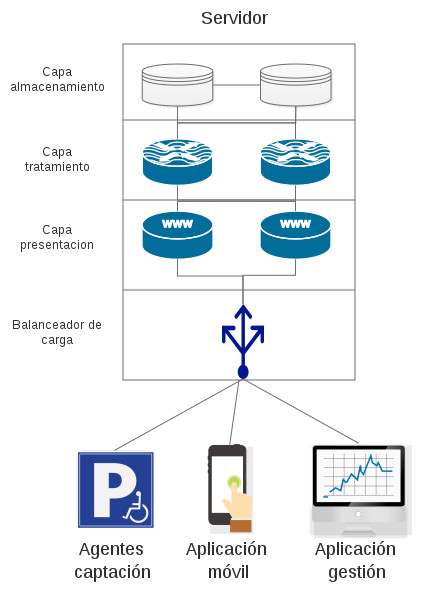
\includegraphics[width=0.5\textwidth]{imagenes/esquema_sistema.jpg}
	\caption{Esquema SGA ideal}
	\label{esquema_sga_ideal}
\end{figure}
\begin{itemize}
	\item en el servidor, ubicado en un centro de procesamiento de datos (CPD), se almacenan, tratan y sirven o reciben datos del resto de dispositivos (parte superior de la figura \ref{esquema_sga_ideal}).
	\item los agentes de captación de datos comprueban el estado de la plaza de aparcamiento y hacen peticiones al servidor para que actualice los datos almacenados en el sistema.
	\item la aplicación móvil muestra al usuario la disponibilidad de los aparcamientos en base a la información almacenada y servida por el servidor.
	\item la aplicación de gestión administra el sistema incluyendo plazas, usuarios, mostrando estadísticas o recibiendo alertas, dependiendo del rol del administrador.
\end{itemize}
